\documentclass[beamer,dvipsnames]{standalone}

\usepackage{tikz}
\usetikzlibrary{positioning}
\usetikzlibrary{shapes}


\definecolor{darkgreen}{RGB}{0,128,80}


\begin{document}

\begin{standaloneframe}

\begin{tikzpicture}[
	arrow double line/.style={
		double distance = 20pt,
	 		shorten <= 11, 	
	 		shorten >= 16,
	 		very thick,
		postaction = {
	  		draw = white,
		line width = 20pt,
		shorten <=-.1pt,
		shorten >=-.1pt,	
		},
		postaction = {
		   	decorate, 
		   	decoration = {
		   		markings, 
		   		mark=at position 0 with {
		   			\arrow[xshift=26.6pt]{Straight Barb[reversed,length=-1pt 0.7]}
		   		},
		   		mark = at position 1 with {
	    			\arrow[xshift=10.6pt]{Straight Barb[length=-1pt 0.7]}
	    		}
   			}
		}
	},
	every node/.style={
		font=\bfseries
	}
]

	

	\def\InterMsgSpaceVertical{1.2}
		
	\node[] (client) {Client};
	\node[inner sep=0pt, xshift=0.0cm,yshift=1cm] (laptop_icon) at (client) {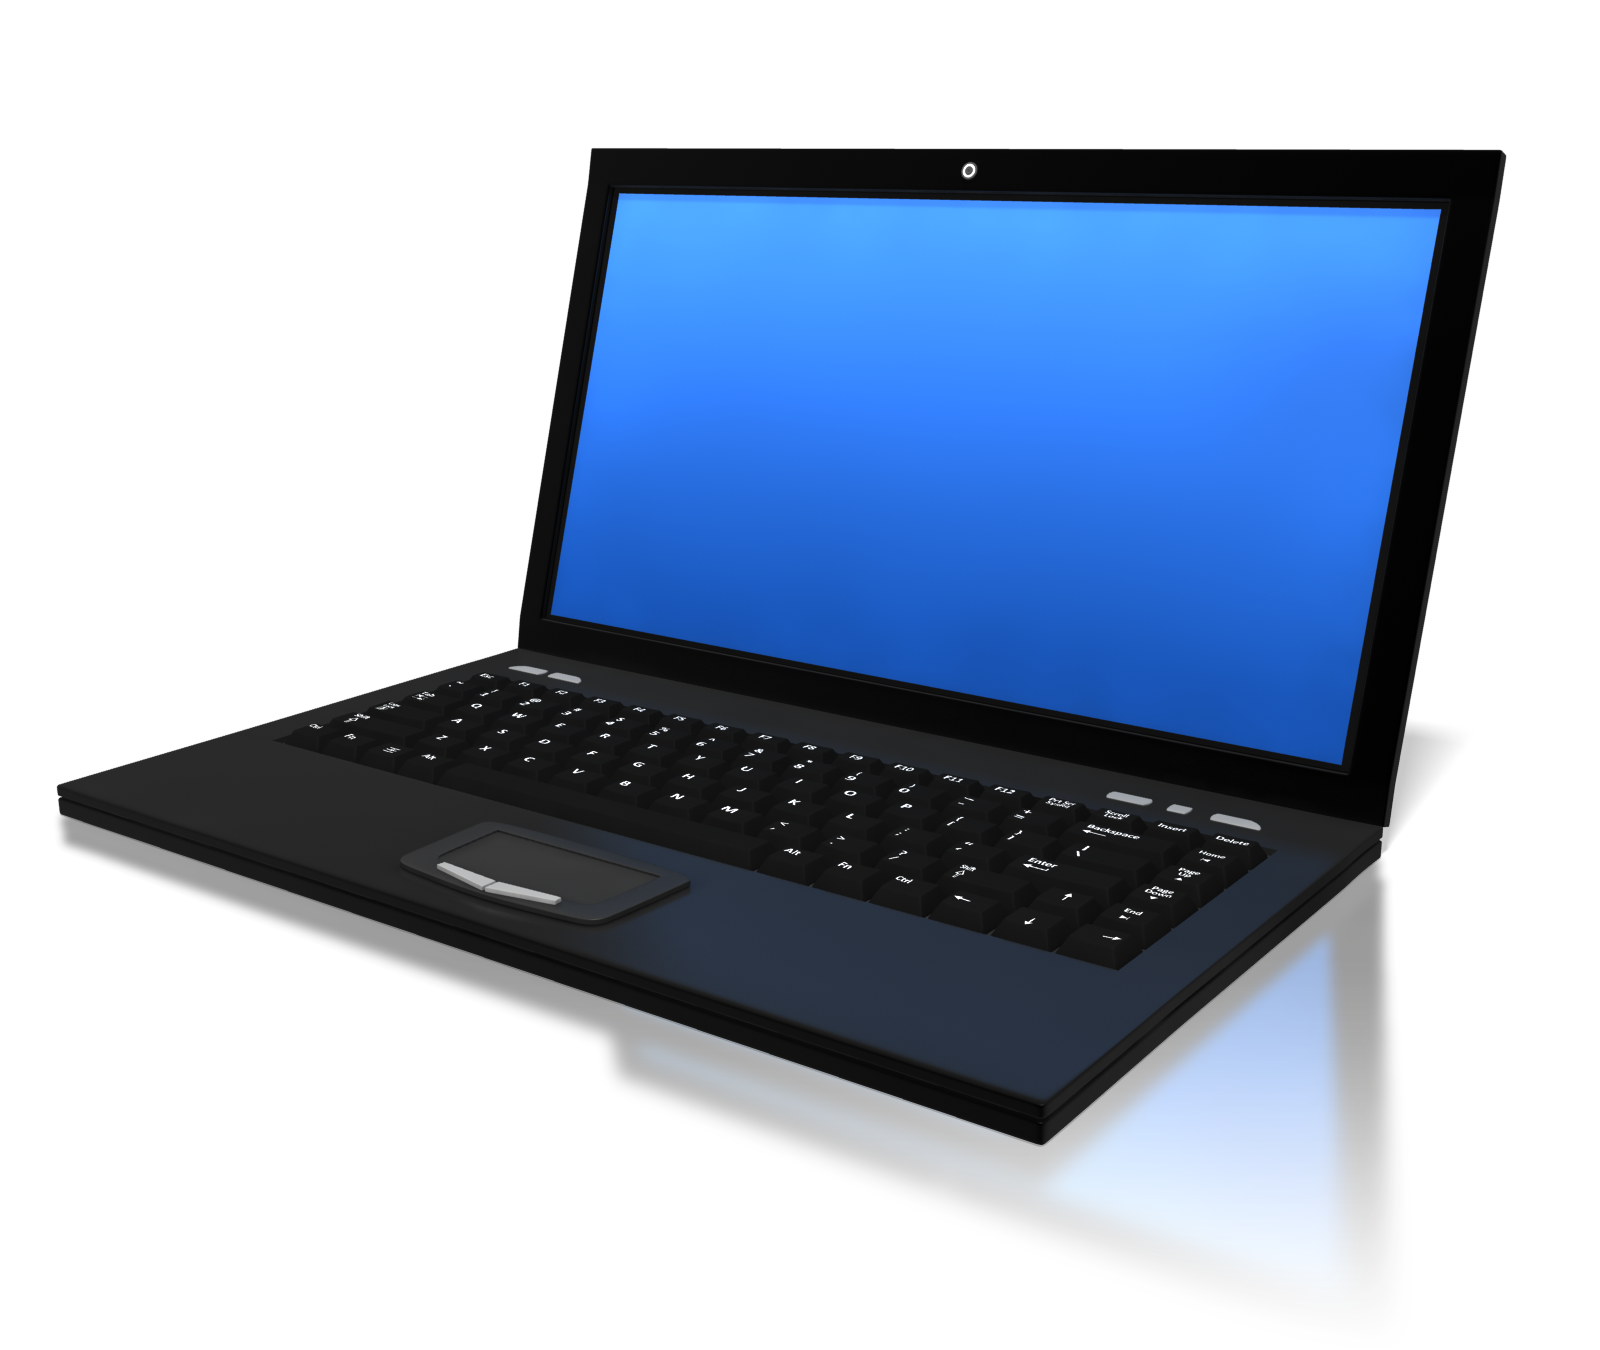
\includegraphics[width=.15\textwidth]{laptop}};
	\node[inner sep=0pt, xshift=1cm,yshift=0.8cm] () at (laptop_icon) {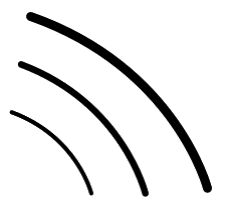
\includegraphics[width=.0487\textwidth]{wireless_signal}};
	
	\node[right = 3 of client] (AP) {Access point};
	\node[inner sep=0pt, xshift=-0.0cm,yshift=1.2cm] (AP_icon) at (AP) {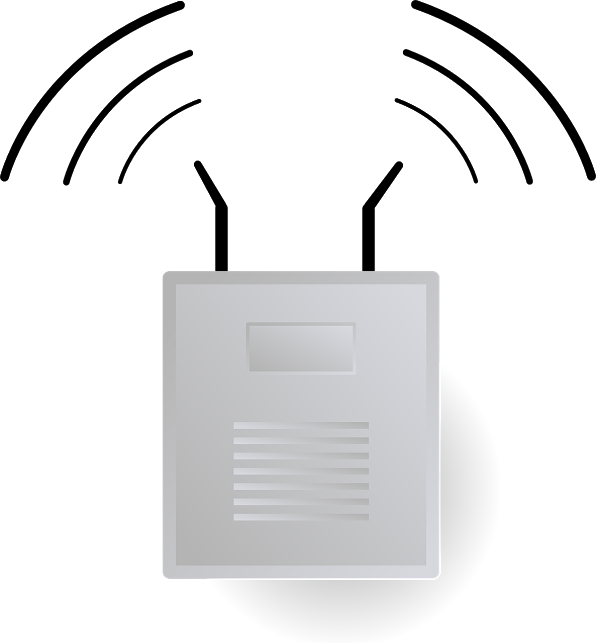
\includegraphics[width=.13\textwidth]{AP}};

	
	\visible<1>{
		\node[above right = 1.06 and 0.4 of client] (key_client) at (client) {
\includegraphics[width=0.07\textwidth]{key_orange}};
		\node[above right = 0.6 and -1.34 of AP] (key_AP) {
\includegraphics[width=0.07\textwidth]{key_orange}};
	}
	
	\visible<3->{
		\node[right = 3 of  AP] (AS) {Server};
		\node[above = -0.1 of AS] (server_icon) {
\includegraphics[width=.1\textwidth]{server}};
		\draw[thick,transform canvas={yshift=0.8cm},shorten >=0.25cm, shorten <=-0.45cm] (AP) -- (AS);
	}

	
	


	
	\visible<4->{
		\node[inner sep=0pt, xshift=0.75cm,yshift=0.75cm] (cert_client) at (laptop_icon) {
\includegraphics[width=.1\textwidth]{cert}};
		\node[inner sep=0pt, xshift=0.3cm,yshift=0.7cm] (server_cert) at (server_icon) {
\includegraphics[width=.1\textwidth]{cert}};
	}
	
%	\visible<3->{
%		\node[inner sep=0pt, xshift=0.5cm,yshift=1.4cm] (key_AP) at (AP) {
\includegraphics[width=0.07\textwidth]{key_blue}};
%		\node[inner sep=0pt, xshift=-0.7cm,yshift=1.4cm] (key_AS) at (AS) {
\includegraphics[width=0.07\textwidth]{key_blue}};
%	}

	
	\coordinate[above = \InterMsgSpaceVertical * 1 of client] (c0) {};
	\coordinate[above = \InterMsgSpaceVertical * 1 of AP] (ap0) {};
	\coordinate[above = \InterMsgSpaceVertical * 1 of AS] (as0) {};
	
	\foreach \i in {1,...,8} {
		\coordinate[below = \InterMsgSpaceVertical * \i of client] (c\i) {};
		\coordinate[below = \InterMsgSpaceVertical * \i of AP] (ap\i) {};
		\coordinate[below = \InterMsgSpaceVertical * \i of AS] (as\i) {};
	}
	
	
	\node[draw, cloud, cloud puffs=15,cloud puff arc=120, aspect=1.5, inner sep=3em, shading = axis,
		top color=blue!1!white,bottom color=blue!8!white,shading angle=20] (cloud) at ([yshift=-0.5cm]ap2) {Internet}; 
	
	\draw[thick] (AP) -- (cloud);
	
%	\draw[thick] (AS) -- (cloud);
	

	
%	\draw[<->, shorten <= 1cm, shorten >= 0.7cm] (c0) to [out=30,in=150] (as0);
	
%	\path[arrow double line, draw] (c0) edge[bend left] node [left] {} (as0);
%	
%	\draw[<->] (AP) -- ([yshift=1cm]AS);
	
%	\draw[arrow double line,red] (c1) -- node (EAP) {EAP method (EAP-TLS)} (as1);
%	
%	\draw[arrow double line,blue] (ap2) -- node[xshift=-2] (AAA) {Key-transport (RADIUS)} (as2);
%	
%	\visible<2-2>{
%		\draw[arrow double line,darkgreen] (c3) -- node[xshift=-2] {Link-layer protocol (IEEE 802.11)} (ap3);
%	}
%	
	

\end{tikzpicture}

\end{standaloneframe}

\end{document}